\documentclass[tikz,border=8pt]{standalone}
% Shared look for every TikZ diagram. Load with \input{../../tools/tikz-style.tex}
\usepackage[sfdefault]{roboto}
\usetikzlibrary{arrows.meta, positioning, shapes.geometric, calc, fit, backgrounds}
\definecolor{cblue}{HTML}{4C78A8}
\definecolor{corange}{HTML}{F58518}
\definecolor{cgreen}{HTML}{54A24B}
\definecolor{cred}{HTML}{E45756}
\definecolor{cpurple}{HTML}{B279A2}
\definecolor{cgrey}{HTML}{6B6B6B}
\tikzset{
  every picture/.style={font=\sffamily, line width=1.2pt},
  box/.style={draw=#1, fill=#1!12, rounded corners=4pt, align=center, inner sep=7pt, minimum height=1.1cm},
  box/.default=cgrey,
  arrow/.style={-{Stealth[length=3mm]}, draw=cgrey, line width=1.4pt},
  title/.style={font=\sffamily\bfseries\Large},
  note/.style={font=\sffamily\small, text=cgrey, align=center},
}
\AtBeginDocument{\hyphenpenalty=10000 \exhyphenpenalty=10000}

% The heading loop with its three outside inputs: the drag torque v enters with the motor torque (load disturbance),
% the output disturbance d moves the heading itself, the sensor noise n corrupts the heading reading.
\begin{document}
\begin{tikzpicture}[every node/.append style={font=\large}]
  \tikzset{sum/.style={circle, draw=cgrey, fill=white, minimum size=0.8cm, inner sep=0pt}}
  \node[align=center] (r) at (0,0) {command\\ $r$};
  \node[sum] (s1) at (1.8,0) {};
  \node[box=cgreen, text width=2.6cm] (C) at (4.6,0) {\textbf{controller}\\ $C(s)$};
  \node[sum] (s2) at (7.5,0) {};
  \node[box=cblue, text width=2.6cm] (P) at (10.3,0) {\textbf{heading plant}\\ $P(s) = \dfrac{1}{0.1\,s^2}$};
  \node[sum] (s3) at (13.2,0) {};
  \node (y) at (15.4,0) {$y$};
  \node[sum] (s4) at (13.2,-3.2) {};
  % inputs
  \node[text=corange, align=center] (v) at (7.5,2.2) {$v$: drag torque\\ \small (load disturbance)};
  \node[text=cred, align=center] (d) at (13.2,2.2) {$d$: output disturbance\\ \small (moves the heading)};
  \node[text=cpurple, align=center] (n) at (13.2,-5.2) {$n$: sensor noise\\ \small (on the reading)};
  \draw[arrow] (r) -- (s1);
  \draw[arrow] (s1) -- node[above] {$e$} (C);
  \draw[arrow] (C) -- node[above, font=\normalsize] {torque $u$} (s2);
  \draw[arrow] (s2) -- (P);
  \draw[arrow] (P) -- (s3);
  \draw[arrow] (s3) -- node[above] {heading} (y);
  \draw[arrow, draw=corange] (v) -- (s2);
  \draw[arrow, draw=cred] (d) -- (s3);
  \draw[arrow, draw=cpurple] (n) -- (s4);
  \draw[arrow] (14.4,0) |- (s4);
  \draw[arrow] (s4) -- node[below] {measured heading $y + n$} (1.8,-3.2) -- (s1);
  \node[font=\Large] at ($(s1.south west)+(-0.05,-0.3)$) {$-$};
  \node[note, font=\normalsize, align=left, anchor=north west] at (-0.6,-4.6)
     {loop transfer function $L = C\,P$; \quad PD: $C(s) = 0.4 + 0.08\,s$};
\end{tikzpicture}
\end{document}
